% Options for packages loaded elsewhere
\PassOptionsToPackage{unicode}{hyperref}
\PassOptionsToPackage{hyphens}{url}
\PassOptionsToPackage{dvipsnames,svgnames,x11names}{xcolor}
%
\documentclass[
  12pt,
]{article}
\usepackage{amsmath,amssymb}
\usepackage{lmodern}
\usepackage{iftex}
\ifPDFTeX
  \usepackage[T1]{fontenc}
  \usepackage[utf8]{inputenc}
  \usepackage{textcomp} % provide euro and other symbols
\else % if luatex or xetex
  \usepackage{unicode-math}
  \defaultfontfeatures{Scale=MatchLowercase}
  \defaultfontfeatures[\rmfamily]{Ligatures=TeX,Scale=1}
\fi
% Use upquote if available, for straight quotes in verbatim environments
\IfFileExists{upquote.sty}{\usepackage{upquote}}{}
\IfFileExists{microtype.sty}{% use microtype if available
  \usepackage[]{microtype}
  \UseMicrotypeSet[protrusion]{basicmath} % disable protrusion for tt fonts
}{}
\makeatletter
\@ifundefined{KOMAClassName}{% if non-KOMA class
  \IfFileExists{parskip.sty}{%
    \usepackage{parskip}
  }{% else
    \setlength{\parindent}{0pt}
    \setlength{\parskip}{6pt plus 2pt minus 1pt}}
}{% if KOMA class
  \KOMAoptions{parskip=half}}
\makeatother
\usepackage{xcolor}
\usepackage[margin = 1.2in]{geometry}
\usepackage{color}
\usepackage{fancyvrb}
\newcommand{\VerbBar}{|}
\newcommand{\VERB}{\Verb[commandchars=\\\{\}]}
\DefineVerbatimEnvironment{Highlighting}{Verbatim}{commandchars=\\\{\}}
% Add ',fontsize=\small' for more characters per line
\usepackage{framed}
\definecolor{shadecolor}{RGB}{248,248,248}
\newenvironment{Shaded}{\begin{snugshade}}{\end{snugshade}}
\newcommand{\AlertTok}[1]{\textcolor[rgb]{0.94,0.16,0.16}{#1}}
\newcommand{\AnnotationTok}[1]{\textcolor[rgb]{0.56,0.35,0.01}{\textbf{\textit{#1}}}}
\newcommand{\AttributeTok}[1]{\textcolor[rgb]{0.77,0.63,0.00}{#1}}
\newcommand{\BaseNTok}[1]{\textcolor[rgb]{0.00,0.00,0.81}{#1}}
\newcommand{\BuiltInTok}[1]{#1}
\newcommand{\CharTok}[1]{\textcolor[rgb]{0.31,0.60,0.02}{#1}}
\newcommand{\CommentTok}[1]{\textcolor[rgb]{0.56,0.35,0.01}{\textit{#1}}}
\newcommand{\CommentVarTok}[1]{\textcolor[rgb]{0.56,0.35,0.01}{\textbf{\textit{#1}}}}
\newcommand{\ConstantTok}[1]{\textcolor[rgb]{0.00,0.00,0.00}{#1}}
\newcommand{\ControlFlowTok}[1]{\textcolor[rgb]{0.13,0.29,0.53}{\textbf{#1}}}
\newcommand{\DataTypeTok}[1]{\textcolor[rgb]{0.13,0.29,0.53}{#1}}
\newcommand{\DecValTok}[1]{\textcolor[rgb]{0.00,0.00,0.81}{#1}}
\newcommand{\DocumentationTok}[1]{\textcolor[rgb]{0.56,0.35,0.01}{\textbf{\textit{#1}}}}
\newcommand{\ErrorTok}[1]{\textcolor[rgb]{0.64,0.00,0.00}{\textbf{#1}}}
\newcommand{\ExtensionTok}[1]{#1}
\newcommand{\FloatTok}[1]{\textcolor[rgb]{0.00,0.00,0.81}{#1}}
\newcommand{\FunctionTok}[1]{\textcolor[rgb]{0.00,0.00,0.00}{#1}}
\newcommand{\ImportTok}[1]{#1}
\newcommand{\InformationTok}[1]{\textcolor[rgb]{0.56,0.35,0.01}{\textbf{\textit{#1}}}}
\newcommand{\KeywordTok}[1]{\textcolor[rgb]{0.13,0.29,0.53}{\textbf{#1}}}
\newcommand{\NormalTok}[1]{#1}
\newcommand{\OperatorTok}[1]{\textcolor[rgb]{0.81,0.36,0.00}{\textbf{#1}}}
\newcommand{\OtherTok}[1]{\textcolor[rgb]{0.56,0.35,0.01}{#1}}
\newcommand{\PreprocessorTok}[1]{\textcolor[rgb]{0.56,0.35,0.01}{\textit{#1}}}
\newcommand{\RegionMarkerTok}[1]{#1}
\newcommand{\SpecialCharTok}[1]{\textcolor[rgb]{0.00,0.00,0.00}{#1}}
\newcommand{\SpecialStringTok}[1]{\textcolor[rgb]{0.31,0.60,0.02}{#1}}
\newcommand{\StringTok}[1]{\textcolor[rgb]{0.31,0.60,0.02}{#1}}
\newcommand{\VariableTok}[1]{\textcolor[rgb]{0.00,0.00,0.00}{#1}}
\newcommand{\VerbatimStringTok}[1]{\textcolor[rgb]{0.31,0.60,0.02}{#1}}
\newcommand{\WarningTok}[1]{\textcolor[rgb]{0.56,0.35,0.01}{\textbf{\textit{#1}}}}
\usepackage{graphicx}
\makeatletter
\def\maxwidth{\ifdim\Gin@nat@width>\linewidth\linewidth\else\Gin@nat@width\fi}
\def\maxheight{\ifdim\Gin@nat@height>\textheight\textheight\else\Gin@nat@height\fi}
\makeatother
% Scale images if necessary, so that they will not overflow the page
% margins by default, and it is still possible to overwrite the defaults
% using explicit options in \includegraphics[width, height, ...]{}
\setkeys{Gin}{width=\maxwidth,height=\maxheight,keepaspectratio}
% Set default figure placement to htbp
\makeatletter
\def\fps@figure{htbp}
\makeatother
\setlength{\emergencystretch}{3em} % prevent overfull lines
\providecommand{\tightlist}{%
  \setlength{\itemsep}{0pt}\setlength{\parskip}{0pt}}
\setcounter{secnumdepth}{5}
\newlength{\cslhangindent}
\setlength{\cslhangindent}{1.5em}
\newlength{\csllabelwidth}
\setlength{\csllabelwidth}{3em}
\newlength{\cslentryspacingunit} % times entry-spacing
\setlength{\cslentryspacingunit}{\parskip}
\newenvironment{CSLReferences}[2] % #1 hanging-ident, #2 entry spacing
 {% don't indent paragraphs
  \setlength{\parindent}{0pt}
  % turn on hanging indent if param 1 is 1
  \ifodd #1
  \let\oldpar\par
  \def\par{\hangindent=\cslhangindent\oldpar}
  \fi
  % set entry spacing
  \setlength{\parskip}{#2\cslentryspacingunit}
 }%
 {}
\usepackage{calc}
\newcommand{\CSLBlock}[1]{#1\hfill\break}
\newcommand{\CSLLeftMargin}[1]{\parbox[t]{\csllabelwidth}{#1}}
\newcommand{\CSLRightInline}[1]{\parbox[t]{\linewidth - \csllabelwidth}{#1}\break}
\newcommand{\CSLIndent}[1]{\hspace{\cslhangindent}#1}
\usepackage{placeins}
\usepackage{fancyhdr}
\usepackage{setspace}
\usepackage{chngcntr}
\usepackage{microtype}
\onehalfspacing
\counterwithin{figure}{section}
\counterwithin{table}{section}
\ifLuaTeX
  \usepackage{selnolig}  % disable illegal ligatures
\fi
\IfFileExists{bookmark.sty}{\usepackage{bookmark}}{\usepackage{hyperref}}
\IfFileExists{xurl.sty}{\usepackage{xurl}}{} % add URL line breaks if available
\urlstyle{same} % disable monospaced font for URLs
\hypersetup{
  colorlinks=true,
  linkcolor={black},
  filecolor={Maroon},
  citecolor={Blue},
  urlcolor={black},
  pdfcreator={LaTeX via pandoc}}

\author{}
\date{\vspace{-2.5em}}

\begin{document}

\pagenumbering{gobble}

\begin{centering}

\vspace{3 cm}

\Huge

{\bf Thesis title}

\vspace{3 cm}

\Large
Author Name

\vspace{3 cm}


\normalsize
Submitted in partial fulfilment of the requirements of the degree of ...

Month Year

\vspace{3 cm}

\normalsize
School of ...

\normalsize
University

\end{centering}

\newpage

\textbf{Declaration}

This is to certify that

\begin{enumerate}
\def\labelenumi{\roman{enumi}.}
\tightlist
\item
  The thesis comprises only my original work except where indicated,
\item
  Due acknowledgement has been made in the text to all other material
  used.
\end{enumerate}

\newpage
\pagestyle{fancy}

\fancyhead[LE,RO]{}
\fancyhead[LO,RE]{}
\renewcommand{\headrulewidth}{0.4pt}
\renewcommand{\footrulewidth}{0pt}

\pagenumbering{roman}

\fancyhead[CO,CE]{Abstract}
\section*{Abstract}
\addcontentsline{toc}{section}{Abstract}

This is an example thesis made with R Markdown.

\newpage
\fancyhead[CO,CE]{Acknowledgements}
\section*{Acknowledgements}
\addcontentsline{toc}{section}{Acknowledgements}

Thank you for reading and good luck. For more information, see
\href{http://rosannavanhespenresearch.wordpress.com}{rosannavanhespenresearch.wordpress.com}.

\newpage
\fancyhead[CO,CE]{Table of Contents}
\setcounter{tocdepth}{2}
\tableofcontents

\newpage
\pagenumbering{arabic}

\newpage
\fancyhead[CO,CE]{Introduction}

\hypertarget{introduction}{%
\section{\texorpdfstring{Introduction\label{label1}}{Introduction}}\label{introduction}}

This is an example introduction. Let's cite someone here (Author 2016).
And in text as well: Author (2013) says that we can cite people in text.
Or we can write the name, and than use the citation thingy to print the
year: Blabla states something about something (2010). Or how about
multiple citations (Author 2013; Author 2016). Or we citation with a
little of text around it (for example see Blabla 2010 pp. 92--93).

We can split up the chapter in subsections:

\hypertarget{subsection}{%
\subsection{Subsection}\label{subsection}}

For example, this is a subsection of the introduction. We can also make
more subsubsections, but they won't be displayed in the table of
contents:

\hypertarget{subsubsection}{%
\subsubsection{Subsubsection}\label{subsubsection}}

There you go, a subsubsection. And just for fun:

\hypertarget{subsubsubsection}{%
\paragraph{Subsubsubsection}\label{subsubsubsection}}

And some text for this subsubsubsection. Let's do another subsection:

\hypertarget{another-subsection}{%
\subsection{Another subsection}\label{another-subsection}}

Some text\ldots{} And finally, a subsection that won't be numbered or
shown in the table of contents:

\subsection*{Kind of invisible subsection}

This section won't be displayed in the table of contents. It also won't
be numbered. Now let's move on to the methods.

\FloatBarrier
\newpage
\fancyhead[CO,CE]{Methods}

\hypertarget{methods}{%
\section{Methods}\label{methods}}

In \autoref{label1} we had look at citations and headings. What about
some equations? Let's put one here:

\begin{equation}
\label{eq-abc}
a + b = c
\end{equation}

You can also write it inline: \(a + b = c\) or use the \$-signs to refer
to a symbol, for example: \(a\) is distance (m).

To refer to the equation in text, you can write: see equation
\ref{eq-abc}. If you use the autoref command, it will automatically
specify what kind of LaTeX object you are referring to, for example: see
\autoref{eq-abc}.

\FloatBarrier
\newpage
\fancyhead[CO,CE]{Results}

\hypertarget{results}{%
\section{Results}\label{results}}

\hypertarget{r-code-output}{%
\subsection{R code output}\label{r-code-output}}

The beauty of R Markdown: including your data analysis directly in the
thesis, so that you update as you go.

Variable\_t has a value of: 12. Note the use of backticks instead of
quotations marks. Backticks can also be used to write code-like text:
\texttt{here\ is\ some\ code} or even do a quick calculation (3 * 6 = :
18 ).

And of course, let's make a plot. You can refer to it in text as normal:
see figure \ref{irisgraph}.

\begin{figure}
\centering
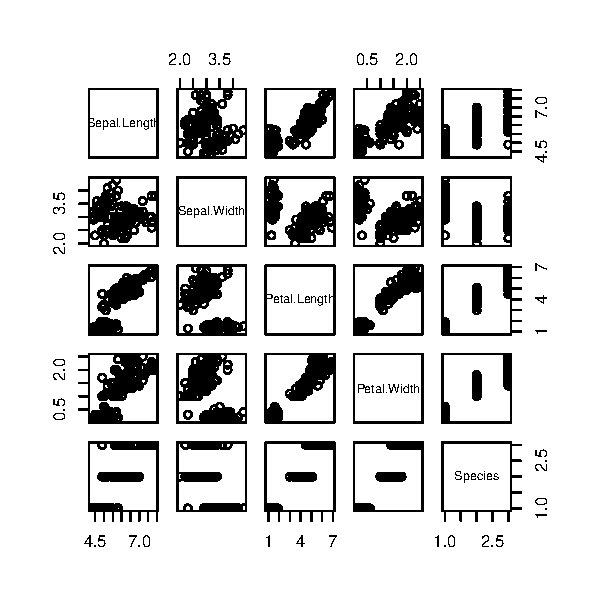
\includegraphics{figures/unnamed-chunk-11-1.pdf}
\caption{Figure caption. \label{irisgraph}}
\end{figure}

\hypertarget{tables}{%
\subsection{Tables}\label{tables}}

This is a \LaTeX  table in an R Markdown document:

\begin{table}
\centering
\caption{This is a table with info}
\label{table-paramvalues}
\begin{tabular}{ p{4cm} p{4cm} p{4cm} }
\hline \\ [-1.5ex]
colname & colname & colname \\ [1ex]
\hline \\ [-1.5ex]
Info & info & info \\ [1ex]
Info & info & info \\ [1ex]
Info & info & info \\ [1ex]
\hline
\end{tabular}
\end{table}

Personally, I prefer \LaTeX tables over R Markdown tables, because you
can tweak them a bit more.

\hypertarget{figures}{%
\subsection{Figures}\label{figures}}

And of course, we can also inlude figures (see figure
\ref{figurelabel}).

\begin{figure}
\centering

\includegraphics{figure1.png}
\caption{This is a figure caption for this beautiful green creation.
\label{figurelabel}}
\end{figure}

\FloatBarrier
\newpage
\fancyhead[CO,CE]{Discussion}

\hypertarget{discussion}{%
\section{Discussion}\label{discussion}}

Finally, the discussion. We had a look at headings and citations in the
introduction, an equation in the methods and figures, r code and tables
in the results. That's it. What will follow now is the list of tables,
list of figures, appendices and references.

\FloatBarrier

\newpage
\fancyhead[CO,CE]{List of Figures}
\addcontentsline{toc}{section}{List of Figures}
\listoffigures

\newpage
\fancyhead[CO,CE]{List of Tables}
\addcontentsline{toc}{section}{List of Tables}
\listoftables

\newpage

\appendix
\section{Appendices}

\subsection{Appendix stuff}

Relabelling the appendix can be a bit tricky. Here I used the standard
\LaTeX syntax `\textbackslash appendix', and using LaTeX labels for
sections instead of R Markdown syntax (i.e.~using
`\textbackslash section' and `\textbackslash subsection' instead of `\#'
and `\#\#'). This automatically produces labels `A.1', `A.2', etc. I
came up with doing it this way during the last two days before handing
in my thesis, so I'm sure this is not the most elegant way of dealing
with the appendices, but it works.

\subsection{Code example}

\begin{Shaded}
\begin{Highlighting}[]
\NormalTok{By setting eval }\OtherTok{=} \ConstantTok{FALSE}\NormalTok{ and echo }\OtherTok{=} \ConstantTok{TRUE}\NormalTok{, }
\NormalTok{the actual code will be displayed but not run.}
\end{Highlighting}
\end{Shaded}

\FloatBarrier
\newpage
\fancyhead[CO,CE]{References}

\hypertarget{references}{%
\section*{References}\label{references}}
\addcontentsline{toc}{section}{References}

\hypertarget{refs}{}
\begin{CSLReferences}{1}{0}
\leavevmode\vadjust pre{\hypertarget{ref-Author2013}{}}%
Author, A. (2013). Another example article with a title. \emph{Journal
of Examples}, \textbf{2}, 21--23.

\leavevmode\vadjust pre{\hypertarget{ref-Author2016}{}}%
Author, T. (2016). This is an example article with a very boring name.
\emph{Journal of Examples}, \textbf{9}, 67--70.

\leavevmode\vadjust pre{\hypertarget{ref-Blabla2010}{}}%
Blabla, B. (2010). It is raining outside. \emph{Journal of Examples},
\textbf{4}, 90--97.

\leavevmode\vadjust pre{\hypertarget{ref-Example1999}{}}%
Example, T. (1999). This is an exmaple article not cited in the text.
\emph{Journal of Examples}, \textbf{4}, 1--9.

\leavevmode\vadjust pre{\hypertarget{ref-Example2000}{}}%
Example, O. (2000). This is another exmaple article not cited in the
text. \emph{Journal of Examples}, \textbf{7}, 28--32.

\end{CSLReferences}

\end{document}
